%%%%%%%%%%%%%%
% LECTURE 17 %
%%%%%%%%%%%%%%
\vspace{1cm}

\noindent\lecture{17}{04/12/2021}

\vspace{0.5cm}

\noindent Riprendiamo il discorso che stavamo affrontando la volta scorsa. L'hamiltoniana $\tilde{H}$ in RWA è indipendente dal tempo, perciò l'evoluzione temporale dello stato generico ruotato è molto semplice
\begin{equation}\label{to_exp_H_tilde}
    \ket{\tilde{\psi}(t)} = e^{-i \tilde{H} t} \ket{\tilde{\psi}(0)} \, .
\end{equation}
In realtà avremmo potuto fin dall'inizio scrivere l'evoluzione temporale dello stato $\ket{\psi (t)}$ non ruotato, utilizzando l'hamiltoniana \eqref{H_no_approx}: abbiamo deciso di non intraprendere quella strada poiché l'espressione dell'operatore unitario che descrive l'evoluzione temporale per $H$ dipendenti dal tempo è abbastanza complicata. 

\noindent Dato che ci serve nella \eqref{to_exp_H_tilde} l'esponenziazione di $\tilde{H}$, esplicitiamo in \eqref{H_tild_RWA} le matrici $\sigma_1$ e $\sigma_2$ (da $\sigma_+$ e $\sigma_-$) e riscriviamo gli esponenziali in termini di seno e coseno: in questo modo otteniamo la seguente combinazione lineare di matrici di Pauli
\begin{equation*}
    \tilde{H} = - \frac{1}{2} \left( \Delta \sigma_3 + A \cos \phi \sigma_1 - A \sin \phi \sigma_2 \right) \equiv -\frac{\Omega}{2} \vec n \cdot \vec \sigma \, ,
\end{equation*}
dove 
\begin{equation}\label{n_dir}
    \vec n = \frac{1}{\Omega} (A \cos \phi, - A \sin \phi, \Delta) \quad \text{con} \quad \Omega = \sqrt{A^2 + \Delta^2} \, ;
\end{equation}
si noti che $\vec n$ è correttamente normalizzato dimodoché $\abs{\vec n} = 1$. La frequenza $\Omega$ è chiamata \textbf{frequenza di Rabi}\footnote{Molti libri usano differenti convenzioni sul significato di tale frequenza. Indipendentemente da ciò, la cosa importante è che l'oscillazione del qubit è controllata da $\Omega$.} e controlla l'oscillazione del qubit. Quindi l'operatore di evoluzione temporale diventa 
\begin{equation}\label{rotation_Omega}
    e^{-i \tilde{H} t} = e^{i \frac{\Omega}{2} \vec n \cdot \vec \sigma t} \, ;
\end{equation}
(la presenza del fattore $1/2$ è comune quando sono presenti le matrici di Pauli). La relazione precedente è esattamente analoga all'operatore \eqref{rotation_n_lambda}, introdotto nella Sezione \ref{sec:gate} riguardante i gate agenti su singoli qubit: la più generale matrice unitaria $2 \times 2$ (a meno di una fase globale) può essere infatti scritta proprio come l'operatore $R_{\vec n}(\gamma)$, ossia
\begin{equation*}
    R_{\vec{n}}(\gamma) = e^{-i \frac{\gamma}{2} (\vec n \cdot \vec \sigma)} \, .
\end{equation*}
Questo operatore va interpretato come una rotazione del qubit lungo la sfera di Bloch: l'evoluzione temporale $R_{\vec n}(- \Omega t)$ effettua una rotazione di angolo $-\Omega t$ attorno alla direzione individuata dal vettore $\vec n$ scritto in precedenza. È bene notare che la direzione attorno a cui avviene questa precessione è specificata dai parametri che individuano i dettagli dell'interazione con la radiazione esterna oscillante, come $\omega_d$, $A$ e $\phi$, ma anche dalla frequenza di oscillazione del qubit stesso ($\omega_q$).  

\noindent Prima di dare uno sguardo concreto alla sfera di Bloch, ricordiamo che per scrivere l'esponenziale di una combinazione lineare di matrici di Pauli è possibile usare la seguente formula:
\begin{equation}\label{formula_for_Rabi}
    R_{\vec{n}}(\gamma) = e^{-i \frac{\gamma}{2} (\vec n \cdot \vec \sigma)} = \mathbb{I} \cos \! \left( \frac{\gamma}{2} \right) - i \sin \! \left( \frac{\gamma}{2} \right) \left( \vec \sigma \cdot \vec n \right) \, .
\end{equation}

\begin{proof}
    Ricordando la serie dell'esponenziale, la proprietà $(\vec \sigma \cdot \vec n)^2 = \mathbb{I}$ e la serie di seno e coseno avremo:
    \begin{align*}
        R_{\vec{n}}(\gamma) &= \sum_{k=0}^\infty \frac{1}{k!} \left( -\frac{i}{2} \gamma \vec n \cdot \vec \sigma \right)^k \\
        &= \sum_{k=0}^\infty \frac{1}{(2k)!} \left( -\frac{i}{2} \gamma \vec n \cdot \vec \sigma \right)^{2k} + \sum_{k=0}^\infty \frac{1}{(2k + 1)!} \left( -\frac{i}{2} \gamma \vec n \cdot \vec \sigma \right)^{2k+1} \\
        &= \mathbb{I} \sum_{k=0}^\infty \frac{(i)^{2k}}{(2k)!} \left( \frac{\gamma}{2} \right)^{2k} -i (\vec n \cdot \vec \sigma) \sum_{k=0}^\infty \frac{(i)^{2k}}{(2k+1)!} \left( \frac{\gamma}{2} \right)^{2k+1} \\
        &= \mathbb{I} \cos \! \left( \frac{\gamma}{2} \right) - i \sin \! \left( \frac{\gamma}{2} \right) \left( \vec \sigma \cdot \vec n \right) \, .
    \end{align*}
\end{proof}

\noindent La \eqref{formula_for_Rabi} è molto utile quando si vogliono affrontare dei conti espliciti. Vediamo per esempio un caso di un esercizio molto semplice in QM:

\begin{esempio}[\textbf{Oscillazioni di Rabi}]
    Supponiamo che il sistema si trovi nello stato iniziale $| \tilde{\psi}(0) \rangle = \ket{0}$ e calcoliamo la probabilità che al tempo $t$ il qubit subisca una transizione $\ket{0} \to \ket{1}$. Ricordando l'espressione \eqref{rotation_Omega} e la formula appena dimostrata avremo
    \begin{equation*}
        P(t)_{0 \to 1} = \abs{\mel{1}{e^{-i \tilde{H} t}}{0}}^2 = \abs{\mel{1}{\cos \! \left( \frac{\Omega}{2} t \right) + i \sin \! \left( \frac{\Omega}{2} t \right) \vec \sigma \cdot \vec n }{0}}^2 \, ;
    \end{equation*}
    il primo termine è nullo, mentre il secondo, ricordando che $\sigma_1 \ket{0} = \ket{1}$ e $\sigma_2 \ket{0} = i \ket{1}$, riceve contributi solamente da $\sigma_1$ e $\sigma_2$. In questo modo possiamo scrivere 
    \begin{align*}
        P(t)_{0 \to 1} &= \abs{i \sin \! \left( \frac{\Omega}{2} t \right) (n_1 + i n_2)}^2 \\
        &= \abs{i \sin \! \left( \frac{\Omega}{2} t \right) \frac{A}{\Omega} e^{-i \phi}}^2 \\
        &= \frac{A^2}{\Omega^2} \sin^2 \! \left( \frac{\Omega}{2} t \right) \, ,
    \end{align*}
    dove nella seconda riga abbiamo usato le componenti di $\vec n$ in \eqref{n_dir}. Inserendo infine l'espressione di $\Omega$ otteniamo la cosiddetta \textbf{formula di Rabi}
    \begin{equation}\label{Rabi_formula}
        P(t)_{0 \to 1} = \frac{A^2}{A^2+\Delta^2} \sin^2 \! \left( \frac{\sqrt{A^2+\Delta^2}}{2} t \right) \, .
    \end{equation}
    
    \begin{figure}[!hb]
    \centering
    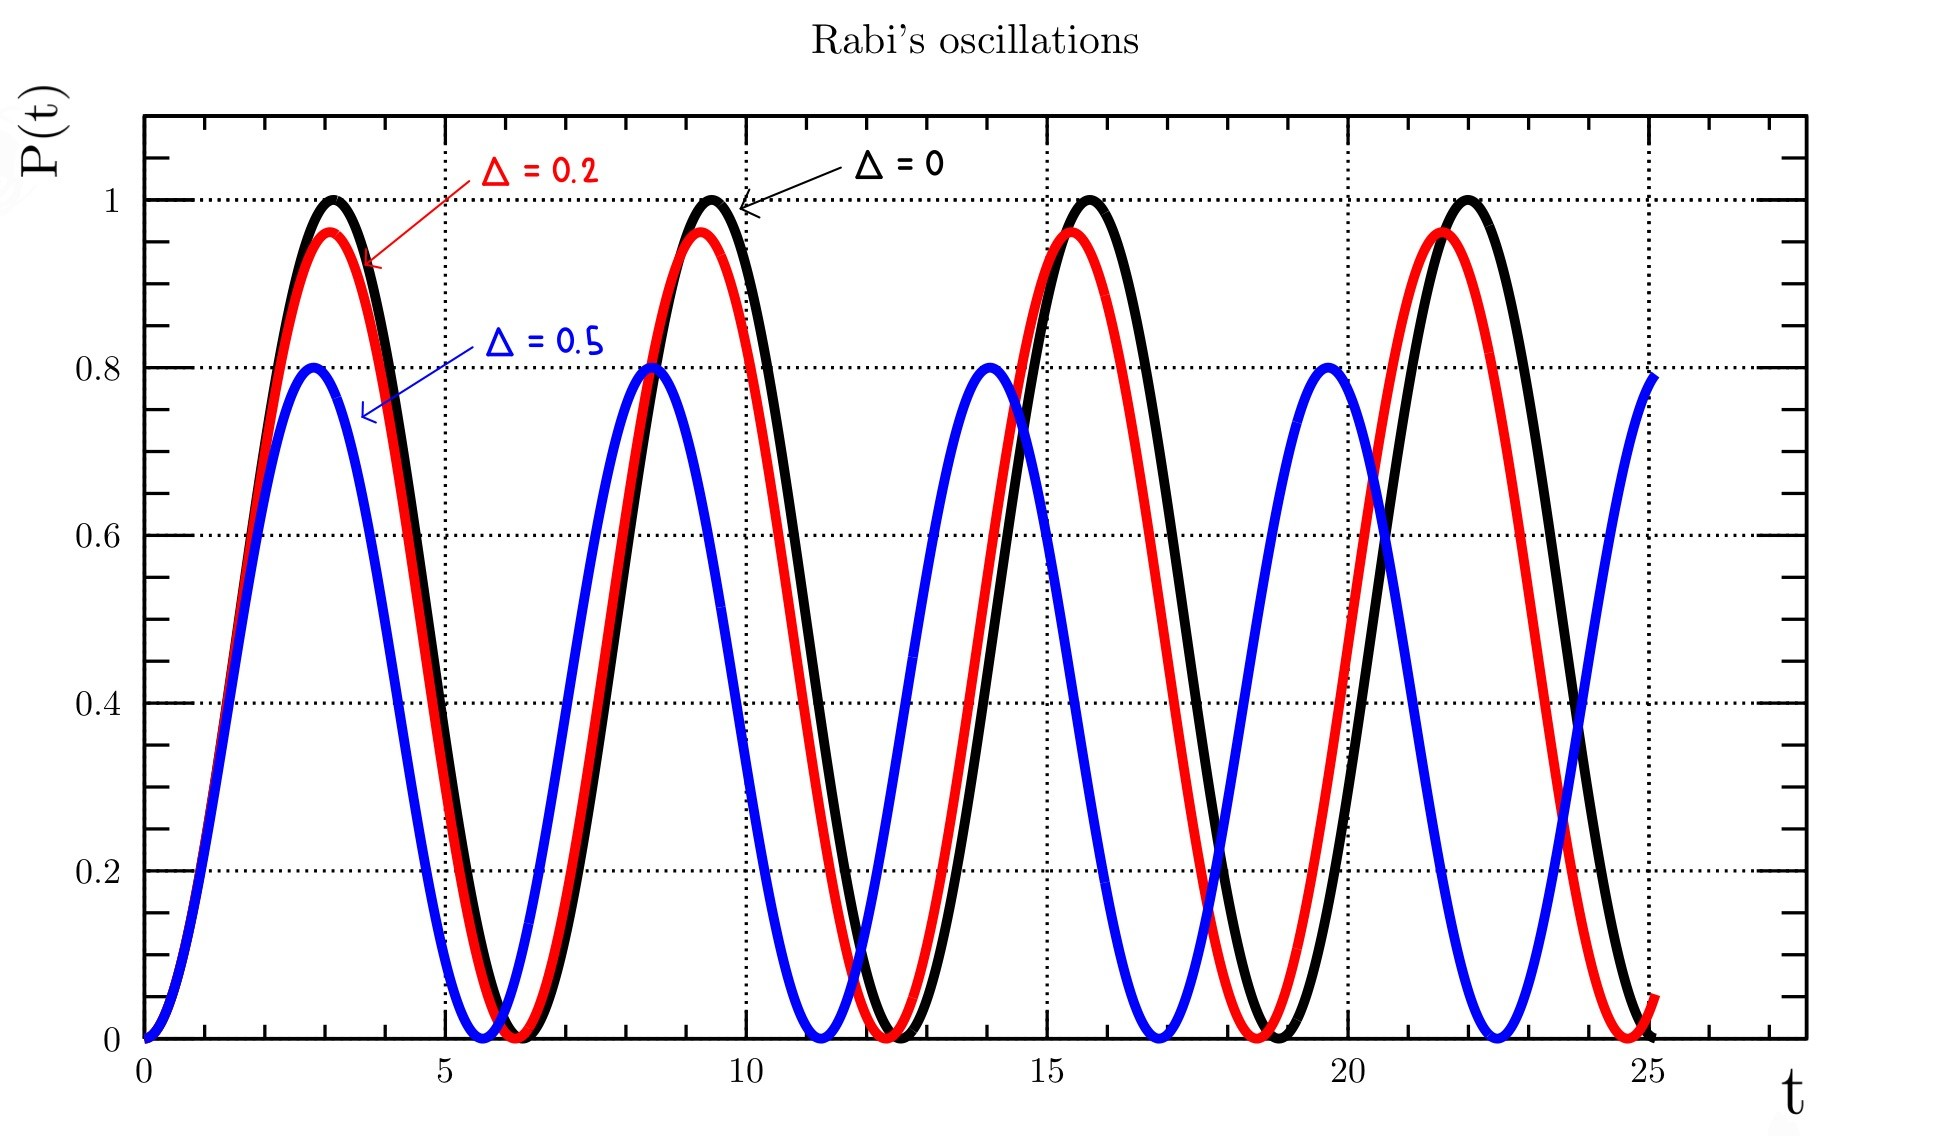
\includegraphics[scale=0.302]{images/Rabi.jpg}
    \caption{Oscillazioni di Rabi per $A = 1$. È evidente come la probabilità del sistema oscilli allo scorrere del tempo. Più il sistema è vicino alla risonanza ($\Delta = 0$), più vicino ad 1 saranno i picchi e quindi maggiore sarà la probabilità di trovare il sistema in $\ket{1}$.}
    \label{fig:Rabi}
    \end{figure}
    
    \noindent Ricapitolando, la \eqref{Rabi_formula} ci fornisce la probabilità al tempo $t$ che applicando una perturbazione esterna oscillante con frequenza $\omega_d$, ampiezza $A$ e detuning $\Delta$ avvenga una transizione $\ket{0} \to \ket{1}$. Si tratta di un risultato molto importante e spesso presente in diversi rami della fisica. 
    
    \noindent Facendo un grafico della probabilità \eqref{Rabi_formula} in funzione del tempo si ottiene la Figura \ref{fig:Rabi}. 
\end{esempio} 

\noindent Cerchiamo ora di visualizzare che cosa accade dal punto di vista della sfera di Bloch. Ricordando la \eqref{rotation_RWA} possiamo scrivere lo stato non ruotato come
\begin{equation*}
    \ket{\psi(t)} = U^\dag (t) \ket{\tilde{\psi}(t)} \, , \quad \text{dove} \quad U^\dag (t) = e^{\frac{i}{2} \omega_d \sigma_3 t} \, ,
\end{equation*}
in questo modo, inserendo anche la \eqref{to_exp_H_tilde}, possiamo scrivere l'evoluzione temporale dello stato non ruotato
\begin{equation}\label{te_non_rotated}
    \ket{\psi(t)} = e^{\frac{i}{2} \omega_d \sigma_3 t} R_{\vec n}(- \Omega t) \ket{\tilde{\psi}(0)} \, .
\end{equation}
Come già anticipato (vedi Figura \ref{subfig:Bloch_Rabi1}), l'operatore $R_{\vec n}(-\Omega t)$ implementa una rotazione di angolo $-\Omega t$ attorno alla direzione di $\vec n$. Per esempio

\begin{esempio}[\textbf{Rotazione attorno a $z$}]
    Supponiamo una rotazione lungo $z$ implementata dall'operatore $R_z(\gamma) = e^{-\frac{i}{2} \sigma_3 \gamma}$. Ricordando la generica parametrizzazione del qubit in \eqref{generic qubit} avremo
    \begin{align*}
        R_z(\gamma) \ket{\psi} &= \cos \! \left( \frac{\theta}{2} \right) e^{-\frac{i}{2} \gamma} \ket{0} + \sin \! \left( \frac{\theta}{2} \right) e^{\frac{i}{2} \gamma} e^{i \phi} \ket{1} \\
        &= e^{-\frac{i}{2} \gamma} \left[ \cos \! \left( \frac{\theta}{2} \right) \ket{0} + \sin \! \left( \frac{\theta}{2} \right) e^{i(\phi + \gamma)} \ket{1} \right] \, ;
    \end{align*}
    riassorbendo la fase globale abbiamo effettivamente ottenuto che l'operatore $R_{\vec n}(\gamma)$ produce una rotazione lungo $z$ perché il qubit finale è dello stesso tipo di quello iniziale con $\theta \to \theta$ e $\phi \to \phi + \gamma$. 
\end{esempio}

\noindent Che cosa accade per una rotazione lungo una generica direzione $\vec n$? La direzione dipende da $(A, \Omega, \phi)$, quindi per rilevarla sperimentalmente basta variare questi parametri. 

\noindent La situazione in cui $A = 0$ (assenza di una perturbazione  esterna) è abbastanza curiosa: in una tale situazione si potrebbe pensare $R_{\vec n} (- \Omega t) = \mathbb{I}$, quindi sembrerebbe dalla \eqref{te_non_rotated} che rimanga un termine $e^{\frac{i}{2} \omega_d \sigma_3 t}$ di rotazione lungo $z$. In realtà questo risultato è sbagliato perché, quando non c'è alcun campo oscillante, è necessario porre $\omega_d = 0$: dalla \eqref{n_dir} il vettore $\vec n$ non è zero, ma bensì $\vec n = (0, 0, \Delta/\Omega)$, perciò
\begin{equation*}
    R_{\vec n} (-\Omega t) = e^{\frac{i}{2} \Delta \sigma_3 t} = e^{\frac{i}{2} (\omega_q - \omega_d) \sigma_3 t} \, ; 
\end{equation*}
questo significa che lo stato continua a subire una precessione
\begin{equation*}
    \ket{\psi(t)} = e^{\frac{i}{2} \omega_d \sigma_3 t} e^{\frac{i}{2} (\omega_q - \omega_d) \sigma_3 t} \ket{\tilde{\psi}(0)} = e^{\frac{i}{2} \omega_q \sigma_3 t} \ket{\tilde{\psi}(0)} \, .
\end{equation*}
Esiste sempre una precessione lungo $z$ con la frequenza naturale del qubit! Delle volte è utile sbarazzarsi di questa precessione cambiando sistema di coordinate: ad esempio possiamo andare in un sistema di riferimento che ruota come il qubit scegliendo $U(t) = e^{i H_0 t}$; in questo modo è possibile tenere solamente la parte non banale dell'evoluzione temporale eliminando questo effetto di precessione. Spesso il sistema di riferimento scelto dipende da ciò che si vuole fare. 

\begin{figure}[!ht]
	\centering	
	\subfloat[][\label{subfig:Bloch_Rabi1} ]{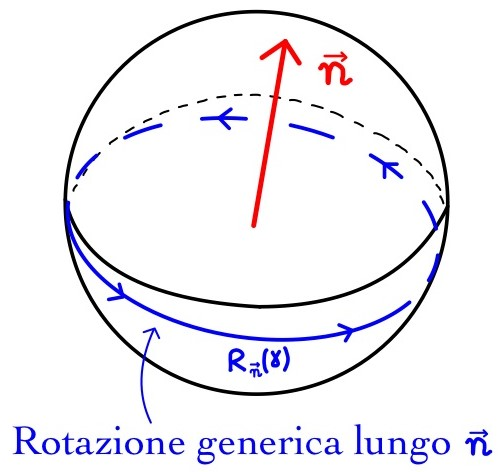
\includegraphics[scale=.4,keepaspectratio]{images/Bloch_Rabi1}} \\
	\subfloat[][\label{subfig:Bloch_Rabi2} ]{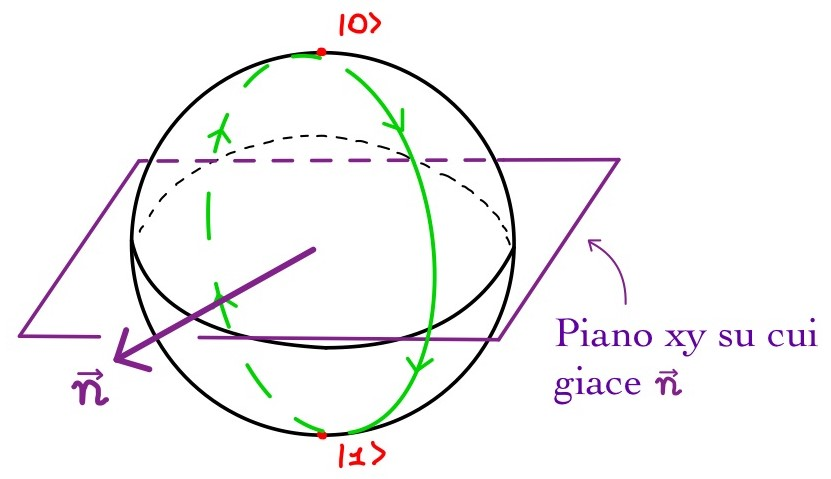
\includegraphics[scale=.4,keepaspectratio]{images/Bloch_Rabi2}} \\
	\subfloat[][\label{subfig:Bloch_Rabi3} ]{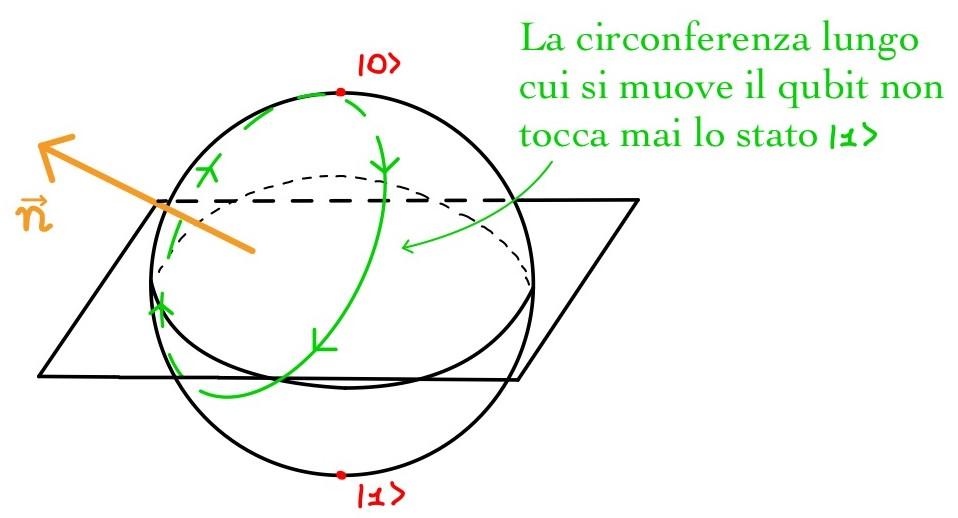
\includegraphics[scale=.4,keepaspectratio]{images/Bloch_Rabi3}}
	\caption{(\ref{subfig:Bloch_Rabi1}) L'operatore $R_{\vec n}(\gamma)$ implementa una generica rotazione attorno ad $\vec n$ lungo la superficie della sfera di Bloch. (\ref{subfig:Bloch_Rabi2}) Alla risonanza, $\vec n$ giace nel piano $xy$, quindi per determinati tempi vi è la certezza che il qubit si trovi in $\ket{1}$. (\ref{subfig:Bloch_Rabi3}) Per $\vec n$ generico non si ha mai la certezza che il qubit si trovi in $\ket{1}$.}
    \label{fig:Bloch_Rabi}
\end{figure}

\noindent Per capire meglio il significato della rotazione di Figura \ref{subfig:Bloch_Rabi1} immaginiamo che il qubit parta nello stato $\ket{0}$. In regime di risonanza ($\Delta = 0$) avremo $\vec n = (\cos \phi, - \sin \phi, 0)$, perciò l'asse di rotazione giace nel piano $xy$ (si consideri la Figura \ref{subfig:Bloch_Rabi2}): geometricamente, il qubit ruota con frequenza $\Omega$ lungo la circonferenza evidenziata in verde, ossia nel piano perpendicolare ad $\vec n$, andando continuamente avanti e indietro da $\ket{0}$ ad $\ket{1}$ (si pensi alla probabilità di Figura \ref{fig:Rabi}). Ci saranno tempi particolari in cui il qubit si trover\`a con certezza in $\ket{1}$.

\noindent Per quale ragione invece per $\Delta \neq 0$ la probabilità non è mai 1? Dalle relazioni \eqref{n_dir}, il vettore $\vec n$ presenta 3 componenti non nulle per $\Delta \neq 0$ quindi, partendo da $\ket{0}$, la circonferenza lungo la quale il qubit si muove non raggiunge mai $\ket{1}$! (si pensi alla Figura \ref{subfig:Bloch_Rabi3}). Ovviamente dalle leggi della QM sappiamo che ci sarà sempre della probabilità che la misura restituisca $\ket{1}$, tuttavia per nessun tempo si avrà la certezza che il qubit si trovi in quello stato. Dal punto di vista pratico è possibile utilizzare questa perturbazione esterna oscillante per muovere arbitrariamente il qubit sulla sfera di Bloch e invertire lo stato dimodoché oscilli continuamente $\ket{0} \leftrightarrow \ket{1}$. 

\noindent Cosa succede quando la perturbazione non è periodica? Una tale situazione è parametrizzata da un campo esterno proporzionale a $f(t) \cos (\omega_d t + \phi_0)$, dove $f(t)$ è un'opportuna funzione dipendente dal tempo. Per svolgere dei conti espliciti è necessario utilizzare il formalismo della teoria delle perturbazioni dipendenti dal tempo: il punto fondamentale è che la fisica rimane la stessa! L'oscillazione è modulata da $f(t)$ perciò è sempre possibile scegliere opportunamente questa funzione e le frequenze in maniera tale che si abbia una situazione in cui, per un dato tempo $t$, il qubit si ritrovi con certezza in $\ket{1}$; in questo modo il tempo può essere scelto arbitrariamente per manipolare il qubit a piacimento. 










\section{Accoppiamento qubit - cavità QED}\label{sec:int_qubit_CQED}
L'accoppiamento di un qubit con un campo elettromagnetico (classico) esterno oscillante può essere essenzialmente utilizzato per creare tutti i gate agenti sui singoli qubit. I gate agenti su più qubit (quelli che creano entanglement tra stati), invece, sono più complessi da realizzare: alcuni di essi possono essere costruiti a partire da situazioni simili a quelle studiate nella scorsa sezione, tuttavia la maggior parte sono realizzati tramite l'accoppiamento di un qubit con un campo elettromagnetico quantizzato. Cerchiamo di approfondire questo discorso. 

\noindent L'elettrodinamica quantistica della cavità (\textbf{Cavity QED}) è un campo di studio che si focalizza su un regime che coinvolge l'accoppiamento di singoli atomi con solo alcuni (pochi) modi ottici. Sperimentalmente, ciò è reso possibile collocando singoli atomi all'interno di cavità ottiche. Poiché all'interno della cavità esistono solo uno o due modi elettromagnetici, e ciascuno di questi ha un'intensità di campo elettrico molto elevata, l'accoppiamento tra il dipolo dell'atomo e il campo è molto intenso. I due principali componenti sperimentali di un sistema QED a cavità sono la cavità elettromagnetica e l'atomo; quest'ultimo, il quale modellizza il qubit, interagisce con alcuni fotoni della cavità, perciò è evidente che dobbiamo considerare un'hamiltoniana che coinvolge una radiazione quantizzata. 

\noindent Nel contesto dell'ottica quantistica si costruisce un tale sistema considerando una cavità Fabry-Perot costituità da una serie di specchi che permettono di intrappolare dei fotoni: il campo elettromagnetico che si genera dalle riflessioni dei fotoni sugli specchi è molto intenso, ma si riescono a selezionare alcuni modi di frequenza $\omega_c$ (pedice $c$ per cavità) ben precisi (o multipli di tale frequenza). Un sistema di questo tipo diventa molto simile alla radiazione di corpo nero perché l'atomo (qubit) nella cavità QED può scambiare e riassorbire fotoni se la frequenza del qubit è simile a quella della cavità, ossia $\omega_q \sim \omega_c$. In generale se i fotoni non possono uscire e l'atomo assorbe alcuni di essi con frequenze ben precise, allora il sistema necessita una completa trattazione in QM. Ovviamente i fotoni possono uscire attraverso delle emissioni spontanee (ricordiamo che c'è sempre qualche perdita e decoerenza).

\noindent L'hamiltoniana totale del sistema, il quale è costituito dal qubit e dalla cavità, sarà descritta da
\begin{equation}\label{eq:ham-cav-qub-free}
    \hat H_0 = -\frac 12 \omega_q\hat \sigma_3+\omega_c\left(\hat a^\dagger \hat a +\frac 12\right) \, ,
\end{equation}
dove in questo caso, nel secondo termine, stiamo descrivendo un solo modo ottico perché nella maggior parte delle situazioni se ne riescono ad eccitare molto pochi; avendo un unico modo del campo e.m. allora, nella trattazione che segue, assumeremo che l'eccitazione dei fotoni coinvolgerà sempre fotoni dello stesso modo ottico dato dagli operatori $\hat{a}$ e $\hat{a}^\dag$. L'hamiltoniana precedente non è nient'altro che l'hamiltoniana libera che descrive contemporaneamente e indipendentemente il qubit e la cavità. Per descrivere la parte interagente del sistema assumiamo un'interazione con il dipolo dell'atomo, quindi introduciamo l'hamiltoniana
\begin{equation}\label{eq:ham-cav-qub-int}
    \hat H_I=\vec d \cdot \vec E \, ,
\end{equation}
dove $\vec d$ dipende dalle interazioni concrete che hanno luogo\footnote{Questo vettore è la posizione se il qubit è costruito da un atomo, altrimenti è lo spin se il qubit è realizzato da un sistema con spin. Similmente, il campo è elettrico nel primo caso, altrimenti è magnetico per l'accoppiamento con lo spin.}, ma allo stesso tempo fornisce i generici elementi di matrice per le transizioni $\ket 0 \rightarrow \ket 1$ e $\ket 1 \rightarrow \ket 0$; $\vec E$ è ovviamente il campo elettrico. Dato che il campo è quantizzato possiamo utilizzare il risultato ottenuto alla fine della Sezione \ref{sec:quantized_em}, cioè
\begin{equation}\label{eq:em-quant.}
    \hat{\vec E} = \vec E_0\left(\hat a e^{i\vec k \cdot \vec x - i \omega t} + \hat a^\dagger e^{-i\vec k \cdot \vec x + i \omega t}\right) \, .
\end{equation}
Diamo uno sguardo alla relazione \eqref{eq:em-quant.}, in particolar modo alla dipendenza spaziale e temporale. Per quanto riguarda la prima, usando l'approssimazione di dipolo, se consideriamo per i fotoni lunghezze d'onda grandi\footnote{Tipicamente la lunghezza d'onda dei fotoni non è così lontana dalla lunghezza d'onda di risonanza del qubit, la quale rimane comunque molto più grande delle dimensioni atomiche.} rispetto alle dimensioni atomiche del sistema, possiamo trascurare la dipendenza spaziale. Un discorso analogo può essere fatto anche per la dipendenza temporale: nel momento in cui si va a quantizzare il campo e.m. di un sistema che assumiamo isolato, l'hamiltoniana che si realizza è solitamente indipendente dal tempo e quindi può essere costruita rispetto a un certo riferimento temporale che, per semplicità, facciamo coincidere con $t=0$. Sotto queste due assunzioni, la \eqref{eq:em-quant.} può essere riscritta come
\begin{equation*}
    \hat{\vec E} = \vec E_0\left(\hat a + \hat a^\dagger\right) \, .
\end{equation*}
Inserendo questo risultato nella \eqref{eq:ham-cav-qub-int} avremo che 
\begin{equation}\label{eq:ham-cav-qub-int2}
    \hat H_I=g\hat\sigma_1\left(\hat a + \hat a^\dagger\right)\, ,
\end{equation}
dove $g$ è la costante di accoppiamento dell'interazione tra il qubit e la radiazione e, anziché prendere gli elementi di matrice dell'operatore $\vec d$ tra gli stati dei qubit (dipendono da molti fattori, come ad esempio i livelli energetici che scegliamo dalle regole di selezione), consideriamo una generica matrice hermitana $2 \times 2$ che, come sappiamo, può essere scritta in termini di una combinazione lineare delle matrici di Pauli. 
Tra tutte le possibili scelte prendiamo, senza perdita in generalità, $\hat \sigma_1$. Ovviamente possiamo fare scelte diverse, come ad esempio $\hat{\sigma_2}$, ma ogni opzione darà sempre un risultato fisico simile.

\noindent A questo punto possiamo mettere insieme la \eqref{eq:ham-cav-qub-free} e la \eqref{eq:ham-cav-qub-int2} per scrivere l'hamiltoniana completa del sistema
\begin{equation}\label{H_da_riscrivere_4}
    \hat H = -\frac 12 \omega_q\hat \sigma_3+\omega_c\left(\hat a^\dagger \hat a +\frac 12\right) + g\hat\sigma_1\left(\hat a + \hat a^\dagger\right) \, ;
\end{equation}
sottolineiamo nuovamente che la differenza principale rispetto al caso della sezione precedente è che qui il campo elettrico è quantizzato, cosa che si riflette con la presenza degli operatori $\hat{a}$ e $\hat{a}^\dag$.

\noindent Ancora una volta, scriviamo $\hat{\sigma}_1$ usando le definizioni di $\hat \sigma_+$ e $\hat \sigma_-$ in \eqref{sigma_+_-}: è evidente che $\hat \sigma_+ \ket{1} = \ket{0}$ e $\hat \sigma_- \ket{0} = \ket{1}$, quindi la prima matrice agisce come operatore di abbassamento sullo stato del qubit, ossia  $\ket{1} \to \ket{0}$, mentre la seconda come operatore di innalzamento $\ket{0} \to \ket{1}$. Se scriviamo $\hat\sigma_1 = \hat\sigma_++\hat\sigma_-$ e ci concentriamo sul solo termine di interazione, avremo quindi
\begin{equation}\label{H_interaz_4}
    \hat H_I = g\big(
    \underbrace{\hat \sigma_+\hat a^\dagger}_{1.}+
    \underbrace{\hat\sigma_-\hat a}_{2.}+
    \underbrace{\hat\sigma_+\hat a}_{3.}+
    \underbrace{\hat\sigma_-\hat a^\dagger}_{4.}
    \big)\, ;
\end{equation}
quale è l'interpretazione di ciascuno di questi 4 termini sottolineati? Tenendo presente che $\hat{a}$ distrugge un fotone, $\hat{a}^\dag$ crea un fotone e che abbiamo posto $\hbar \omega_q = E_1 - E_0$, il loro significato sarà:
\begin{enumerate}
    \item Il qubit emette un fotone e di conseguenza lo stato energetico si diseccita;
    \item Il qubit assorbe un fotone e di conseguenza lo stato energetico si eccita;
    \item Assorbimento di un fotone e diseccitazione del qubit: viene fornita energia $2 \omega_q$;
    \item Emissione di un fotone ed eccitazione del qubit: viene rimossa energia $-2 \omega_q$.
\end{enumerate}
Gli ultimi due processi sono abbastanza insoliti, anche se potrebbero verificarsi se il sistema possiede energia a sufficienza. In teoria delle perturbazioni al primo ordine solamente i primi due processi sono permessi, mentre gli ultimi due sono vietati dalla regola d'oro di Fermi, perciò, anche in una trattazione esatta, hanno una probabilità molto piccola di verificarsi. Possiamo quindi assumere che i primi due termini siano permessi (più probabili) quando siamo vicini alla risonanza, mentre gli ultimi sono soppressi in teoria delle perturbazioni perché hanno una piccola probabilità che accadano: dunque, a meno che $\omega_c$ e $\omega_q$ non siano troppo lontani tra loro, possiamo trascurare gli ultimi due processi. 

\noindent Verifichiamo quanto detto, ancora una volta, con la RWA, ma questa volta prendiamo una strada leggermente diversa, perché è più conveniente scegliere
\begin{equation*}
    \hat U(t) = e^{i\hat H_0 t} \, ,
\end{equation*}
dove $\hat H_0$ non è nient'altro che l'hamiltoniana della \eqref{eq:ham-cav-qub-free} (questa è nota come \textit{rappresentazione di interazione} in teoria delle perturbazioni). Vediamo come cambia la nuova hamiltoniana a seguito dell'azione $\hat U$: se usiamo la \eqref{S_eq_rotated_state} allora è facile vedere che la scelta precedente ci permette di cancellare il termine libero, infatti
\begin{equation*}
    \hat{\tilde{H}} = \hat U \hat H \hat U^\dagger + i\dot{\hat U}\hat U^\dagger=\hat H_0 + \hat U \hat H_I \hat U^\dagger - \hat H_0= \hat U \hat H_I \hat U^\dagger \, .
\end{equation*}
Per calcolare la coniugazione dell'hamiltoniana \eqref{H_interaz_4} è necessario fare uso del Lemma \ref{lemma:lemma_ops}. Ricordando le seguenti regole di commutazione
\begin{align*}
    \comm{\hat H_0}{\hat a^\dagger} &= \omega_c \hat a^\dagger \, , 
    &\comm{\hat H_0}{\hat \sigma_+} &= -\omega_q\hat \sigma_+ \, , \\
    \comm{\hat H_0}{\hat a} &= -\omega_c \hat a \, , &\comm{\hat H_0}{\hat \sigma_-} &= \omega_q\hat \sigma_- \, ,
\end{align*}
possiamo facilmente scrivere che
\begin{equation}\label{RWA_ops_trans}
    \begin{aligned}
    e^{i\hat H_0t} \hat a^\dagger e^{-i\hat H_0t} &= e^{i\omega_ct} \hat a^\dagger \, , \qquad
    &e^{i\hat H_0t} \hat \sigma_+ e^{-i\hat H_0t} &= e^{-i\omega_qt} \hat \sigma_+ \, , \\
    e^{i\hat H_0t} \hat a e^{-i\hat H_0t} &= e^{-i\omega_ct} \hat a \, , \qquad
    &e^{i\hat H_0t} \hat \sigma_- e^{-i\hat H_0t} &= e^{i\omega_qt} \hat \sigma_- \, ;
    \end{aligned}
\end{equation}
in questo modo la coniugazione completa diventa
\begin{equation*}
    \hat{\tilde{H}} = g \Big( 
    \underbrace{e^{i(\omega_c - \omega_q)t}}_{\sim 1}\hat \sigma_+\hat a^\dagger +
    \underbrace{e^{-i(\omega_c - \omega_q)t}}_{\sim 1}\hat \sigma_-\hat a +
    \underbrace{e^{-i(\omega_c + \omega_q)t}}_{\sim e^{-2i\omega_qt}}\hat \sigma_+\hat a +
    \underbrace{e^{i(\omega_c + \omega_q)t}}_{\sim e^{2i\omega_qt}}\hat \sigma_-\hat a^\dag
    \Big)
\end{equation*}
dove abbiamo supposto il regime di risonanza $\omega_c \sim \omega_q$. Gli ultimi due termini, dal momento che presentano delle rapide oscillazioni, sono soppressi in teoria delle perturbazioni e possiamo quindi trascurarli nella RWA, proprio come avevamo discusso nella sezione precedente.

\noindent Ritornando infine all'hamiltoniana \eqref{H_da_riscrivere_4} nel sistema di riferimento non ruotato, possiamo trascurare gli ultimi due termini della \eqref{H_interaz_4} e scrivere quindi la cosiddetta \textbf{hamiltoniana di Jaynes-Cummings}:
\begin{equation}\label{eq:ham-jaynes-cummings}
    \hat H = -\frac{\omega_q}{2}\hat \sigma_3 + \omega_c\left(\hat a^\dagger \hat a + \frac 12\right)+g\left(\hat \sigma_+\hat a^\dagger + \hat \sigma_-\hat a\right) \, .
\end{equation}
Si tratta dell'hamiltoniana che descrive il sistema della cavity QED, ossia un qubit interagente con delle oscillazioni descrivibili dal punto di vista quantistico (non necessariamente fotoni). Nelle sezioni successive, quando verrà trattato il sistema della trappola ionica, considereremo dei fononi, ma l'hamiltoniana rimarrà comunque della stessa forma. Di solito anche per i qubit superconduttivi si utilizzano hamiltoniane di questo tipo.